\documentclass[12pt]{article}

\usepackage[13643]{easymcm}  % Team control number
\usepackage{longtable}
\usepackage{booktabs}
\usepackage{algorithm}
\usepackage{algpseudocode}

\newcommand{\toB}[1]{\color{blue}#1\color{black}}

\problem{A}  % Problem number

\title{Paper Name}  % Title

\begin{document}

\begin{abstract}

	Some random text
	
\end{abstract}

\maketitle
\tableofcontents

\section{Introduction}

	\subsection{Problem Background}
		
		
		
	\subsection{Problem Restatement}
	
		some random text

\section{Dandelion Spread Model}

	\subsection{Assumptions and Justifications}
	
		\begin{enumerate}
			
			\item \textbf{The dandelion is at the midpoint of a square field's edge, which is 100m long.  Seeds that are blown out of the field are neglected.}
			\vspace{-0.125in}
			\begin{description}
				\item[Justification:] According to the problem, the dandelion is adjacent to the field.  It is reasonable that we set the plant on an edge.  Furthermore, we limit our considerations within the field.  We may assume that a river or forest borders the field, so seeds cannot spread outside.
			\end{description}
			
			\item \textbf{The field is open and planar.}
			\vspace{-0.125in}
			\begin{description}
				\item[Justification:] We only consider the case of flat terrain.  This helps us simplify the spread into two dimensions.  Besides, crop fields and grasslands are usually plains.  Dandelion spread in these terrains are of greatest interest.
			\end{description}
			
			\item \textbf{No other plants hinder the spread of dandelions.}
			\vspace{-0.125in}
			\begin{description}
				\item[Justification:] This means \textbf{a.} dandelion seeds are not intercepted by other plants; and \textbf{b.} dandelions do not have to compete with other plants.  To consider other plants, we would have to obtain data about the distribution, morphology, growth habits, etc., of the local plants.  These would make our model too complex.
			\end{description}
			
			\item \textbf{Wind direction is uniformly distributed from 0$^\circ$ to 360$^\circ$.}
			\vspace{-0.125in}
			\begin{description}
				\item[Justification:] \label{assumption:wind} Wind direction is very variable and local wind directions may be different from those at a weather station.  Therefore, we decided not to use the wind direction data we obtained.
				
				Moreover, we do not know on which edge the dandelion is located.  We cannot determine which wind blows the seeds into the field.  If wind direction is uniformly distributed, all directions are equivalent and we can let the dandelion be located on an arbitrary edge.
			\end{description}
			
			\item \textbf{Dandelions do not die.}
			\vspace{-0.125in}
			\begin{description}
				\item[Justification:] Dandelions are resistant to drought and cold temperature.  When they are partly eaten, they can regrow from the taproot.  Therefore, it is relatively difficult for them to die.
				
				The death of dandelions can be caused by \textbf{a.} insects or pathogens; \textbf{b.} humans (through herbicides or other means); or \textbf{c.} extreme weather.  It is likely that dandelions do not encounter natural enemies when it is introduced to a new location, so we decide to neglect a.  For b. and c., we can consider a natural environment with no extreme weather conditions.  
			\end{description}
			
		\end{enumerate}
		
	
	

	
	\subsection{Model Overview}
		
		We consider five environmental factors, as shown in \textbf{Table \ref{tb:vars}}, and we will construct a temperature curve in \textbf{Section \ref{sec:temp}}.  The environment affects dandelion spread in two major ways.  First, wind influences seed dispersal.  We will model this in \textbf{Section \ref{sec:wind}}.  Second, the combined effect of temperature and humidity influences many aspects in dandelion growth.  We will introduce an adaptation factor $k$ for this in \textbf{Section \ref{sec:af}}.  
		
		{
			\fontsize{10}{14}\selectfont
			{
				\begin{longtable}{ccc}
					\caption{Environmental factors}
					\label{tb:vars}\\
					\toprule
					Symbol&Description&Unit\\
					\toprule
					$\mu_T$&Mean temperature&$^\circ$C\\
					$\sigma_T$&Standard deviation of temperature&$^\circ$C\\
					$\mu_W$&Mean wind speed&m/s\\
					$\sigma_W$&Standard deviation of wind speed&m/s\\
					$\mu_H$&Mean humidity&\%\\
					\bottomrule
				\end{longtable}
			}
		}
	
		Our model simulates the spread of dandelions by tracking every single dandelion.  Every dandelion behaves according to a life cycle pattern, which we will model in \textbf{Section \ref{sec:life}}.  
		
		We will introduce several random variables to allow for some natural variation.  These will make it very hard to directly solve or analyze the model.  Therefore, we will use the Monte Carlo method and run the simulation many times.
	
	
	
	\subsection{Temperature Curve}
	\label{sec:temp}
	
		\begin{wrapfigure}{r}{0.475\textwidth}
			\vspace{-0.4cm}
			\centering
			\includegraphics{fig-temperature_curve.pdf}
			\caption{Temperature curve}
			\label{fig:temp}
		\end{wrapfigure}
		
		We assume that the temperature follows a sinusoidal curve, as shown in \textbf{Fig.\ref{fig:temp}}.  We only consider locations in the northern hemisphere, so we further assume that the lowest temperature is reached on Jan.1st, when time $t = 0$.  We observe that the period of the curve is 360 (for convenience, we set each month to 30 days).  Thus, we write the equation as:
		
		\[
			T = -A \cos{\frac{2\pi}{360} t} + B.
		\]
		
		These conditions should be satisfied:
		
		\[
			\mu_T = \frac1{360} \int_0^{360} (-A \cos{\frac{2\pi}{360} t} + B) \, \mathrm{d}t,
		\]
		
		\[
			\sigma_T^2 = \frac1{360} \int_0^{360} \left[ (-A \cos{\frac{2\pi}{360} t} + B) - \mu_T \right] ^2 	\mathrm{d}t.
		\]
		
		Solving for $A$ and $B$, we get
		
		\begin{equation} \label{eq:temp}
			T = -\sqrt2 \sigma_T \cos{\frac{2\pi}{360} t} + \mu_T.
		\end{equation}





	\subsection{Wind and Dispersal}
	\label{sec:wind}
		
		For the \textbf{direction} of seed dispersal, we assume that the seed always follows the direction of the wind, which is uniformly distributed from 0$^\circ$ to 360$^\circ$ according to \textbf{Assumption \ref{assumption:wind}}.  
		
		For the \textbf{distance} of seed dispersal, we consider two types of wind, horizontal wind and updraft (see \textbf{Fig.\ref{fig:dispersal}}).  The seed travels either a ``normal'' distance $s_N$ due to horizontal wind or a ``long'' distance $s_L$ due to updraft.  We take the $\max\{s_N, s_L\}$ for the distance that the seed travels.
		
		\begin{figure}[htbp]
			\centering
			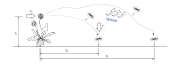
\includegraphics {wind_mode.pdf}
			\caption{Dandelion dispersal distance}
			\label{fig:dispersal}
		\end{figure}
		
		In the case of horizontal wind, we have
		\begin{equation}\label{eq:hwind}
		 \frac{s_N}{v_h} = \frac{h}{v_v},
		\end{equation}
		where $v_h$ is the speed of the horizontal wind, $h$ is the height of the dandelion, and $v_v$ is the vertical component of the velocity of the seed.  $v_h$ follows a normal distribution with $\mu_{v_h} = \mu_W$ and $\sigma_{v_h} = \sigma_W$.  $h$ can be determined for any given plant.  $v_v$ is approximately constant, with value 0.4 m/s.  Thus, we can calculate the value of $s_N$.
		
		\begin{wrapfigure}{r}{0.5\textwidth}
			\vspace{-0.75cm}
			\centering
			\includegraphics{fig-wind_curve.pdf}
			\caption{Cumulative distribution function of\\long-distance dispersal}
			\label{fig:longDistance}
		\end{wrapfigure}
		
		In the case of updraft, we suppose that $s_L$ follows an exponential distribution with cumulative distribution function $\mathrm{P} (s_L < s) = 1 - ae^{-bs}$.  We know $\mathrm{P} (s_L < 0) = 0$.  We also know that the probability of a seed being blown further than 10m is 0.5\%.  Therefore we can obtain
		
		\begin{equation}\label{eq:updraft}
			\mathrm{P} (s_L < s) = 1 - e^{-0.53 s}.
		\end{equation}
		
		Finally, the leafs of dandelions have a radius of around 15cm.  If a seed were to land without falling on the leaf of another dandelion, the dandelion density should be less than $(1/0.15)^2$ = 45 plants/m$^2$.  If a seed arrives at a location whose vicinity has a density greater than this maximum value, the seed fails to land.
		
		
		
		
		
	\subsection{Adaptation Factor}
	\label{sec:af}
		
			We introduce an adaptation factor $k$ using $T$ and $\mu_H$.  Dandelions prefer temperate climates and relatively high humidity.  We divide temperature into three ranks, which respectively indicate that the temperature is very, moderately, or not very suitable for dandelions.  A rank for humidity is obtained in the same way.  On a given day, we calculate $k$ by computing the arithmetic mean of the rank for temperature and humidity and scaling $k$ so that $0 \leq k \leq 1$.
			
			We use $k$ to determine the mean value of some parameters of dandelions, such as the height of the plant.  To allow for some variation, we let the parameters follow normal distributions with
			\begin{equation}\label{eq:k}
				\mu_{\mathrm{parameter}} = \left( \mathrm{worst} + \frac{\mathrm{best} - \mathrm{worst}}4 \right) + k \frac{\mathrm{best} - \mathrm{worst}}2, \,
				\sigma_{\mathrm{parameter}} = \frac{\mathrm{best} - \mathrm{worst}}{12}.
			\end{equation}
			The worst and best values for the relevant parameters will be given in \textbf{Section \ref{sec:life}}.  If the a parameter falls exceeds the worst or best values, it is set to that value.
		
		
		
		
		
	\subsection{Dandelion Life Cycle}
	\label{sec:life}
		
		A dandelion can transfer between 6 states: \textbf{seed}, \textbf{developing}, \textbf{dispersal}, \textbf{inter-dispersal}, \textbf{hold}, and \textbf{dormancy}.
		
		\begin{figure}[htbp]
			\centering
			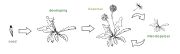
\includegraphics {life_cycle.pdf}
			\caption{Dandelion life cycle}
			\label{fig:lifeCycle}
		\end{figure}
		
		Out of all \textbf{seed}s, only 2\% will successfully germinate.  These seeds will spend 3 days growing into the developing stage.
		
		The \textbf{developing} stage is the stage when the flower is grown and the seeds ripen.  It takes a seed 60--95 days to grow into a flower, and it takes an additional 9--12 days for the seeds on the flower to mature.  The exact duration of this stage is determined by the adaptation factor $k$ (worst = 107, best = 69).
		
		The height of the flower is determined by $k$ (worst = 12, best = 40) when developing finishes.
		
		When $T > 24^\circ$C, only 12.5\% of the flowers bloom and disperse their seeds.  We let dandelions enter dispersal by probability 12.5\% and move the rest into the hold stage.
		
		The \textbf{dispersal} stage lasts 10 days.  A dandelion plant can produce around 10 seed heads per year and it usually flowers twice, so it produces 5 heads every time it flowers.  The number of seeds on each head is determined by $k$ (worst = 150, best = 200).  It takes each head 2 days to disperse its seeds.  The seeds are dispersed per the method stated in \textbf{Section \ref{sec:wind}}.

		The \textbf{inter-dispersal} stage is the stage between two dispersal stages of a plant.  In this stage, dandelions regrow their scapes and flowers.  Since most dandelions that flowered in spring usually flower again in fall, the duration of this stage is set to be half a year, which is 180 days.  
		
		Dandelions can only enter the \textbf{hold} stage when $T > 24^\circ$C.  Flowers are held in buds and dispersal is diminished.  As soon as $T$ falls below $24^\circ$C, flowers can bloom and disperse seeds.  
		
		Dandelions can only enter the \textbf{dormancy} stage when $T < 0^\circ$C.  The temperature is low and it is likely that it snows.  All life activities of dandelions are paused.  As soon as $T$ rises above $0^\circ$C, dandelions resume the stage before it entered dormancy.
		
		
		
		
		
	\subsection{Algorithm}
	
	\subsection{Dandelion Spread Results}
	
		\subsubsection{Simulation Conditions}
		
			We choose 6 locations in the US so that we have a variety of temperature and wind conditions.  AK is cold; CA, DC, and KS are warm; and FL and HI are relatively hot.  AK, DC, and KS have distinct seasons; CA and FL show moderate temperature fluctuations; and HI has very stable temperature.  The wind conditions also exhibit different patterns.  DC has notably large wind speed.  The values of the five environmental factors are listed in \textbf{Table \ref{tb:locs}}.  
			
			{
				\fontsize{10}{14}\selectfont
				{
					\begin{longtable}{ccccccc}
						\caption{Environmental factors for six locations}
						\label{tb:locs}\\
						\toprule
						State&Abbreviation&$\mu_T$ ($^\circ$C)&$\sigma_T$ ($^\circ$C)&$\mu_W$ (m/s)&$\sigma_W$ (m/s)&$\mu_H$ (\%)\\
						\toprule
						Alaska&AK&-0.05&9.08&7.27&1.42&81.46\\
						California&CA&16.20&4.99&6.02&0.90&80.36\\
						District of Columbia&DC&12.64&8.63&13.97&9.51&77.49\\
						Florida&FL&22.11&4.76&6.51&1.71&77.05\\
						Hawaii&HI&22.75&1.40&6.23&0.69&74.64\\
						Kansas&KS&12.58&9.98&8.58&1.55&79.37\\
						\bottomrule
					\end{longtable}
				}
			}
			
			We also have to determine the starting time of simulation.  We run the model with starting dates Jan.\,1st, Feb.\,1st, \ldots, and Dec.\,1st for all 6 locations.  The results for Florida are shown in \textbf{Fig.\ref{fig:start}}.  The dandelion number varies greatly among the runs, but the mean distance is approximately the same.  For each location, the starting date is chosen such that the number of dandelions is maximized.  The number of dandelions corresponding to the chosen dates are marked blue in \textbf{Table \ref{tb:start}}.
			
			\begin{figure}[htbp]
				\centering
				\includegraphics{start_month-number.pdf}
				\caption{Number and mean distance in Florida when simulation starts at different months}
				\label{fig:start}
			\end{figure}
			
			{
				\fontsize{10}{14}\selectfont
				{
					\begin{longtable}{ccccccccccccc}
						\caption{Number at six locations when simulation starts at different dates}
						\label{tb:start}\\
						\toprule
						State&Jan.&Feb.&Mar.&Apr.&May&Jun.&Jul.&Aug.&Sept.&Oct.&Nov.&Dec.\\
						\toprule
						AK&74&79&70&35&44&75&43&49&\color{blue}\textbf{82}&72&74&75\\
						CA&547&567&545&532&585&561&544&\color{blue}\textbf{596}&564&566&581&563\\
						DC&1611&1589&1609&1563&1680&1657&1673&1733&\color{blue}\textbf{1808}&1696&1677&1658\\
						FL&424&417&505&895&\color{blue}\textbf{905}&453&375&384&706&436&435&736\\
						HI&519&329&610&593&586&596&308&543&\color{blue}\textbf{618}&383&385&600\\
						KS&823&276&268&405&548&274&266&\color{blue}\textbf{1067}&287&288&950&834\\
						\bottomrule
					\end{longtable}
				}
			}
			
			
			
		\subsubsection{Results}
		
			We run the model 1000 times for each location.  The resulting frequency histogram for Florida is shown in \textbf{Fig.\ref{fig:freqDand}}.  We can see that both the number and the mean distance follow an approximately normal distribution.  We calculated several statistics for each location, which are displayed in \textbf{Table \ref{tb:numDistribution}} and \textbf{Table \ref{tb:distDistribution}}.
			
			\begin{figure}[htbp]
				\centering
				\includegraphics{number-frequency.pdf}
				\caption{Frequency distribution of number and mean distance in Florida}
				\label{fig:freqDand}
			\end{figure}
			
			We examine the statistics for dandelion number.  For all locations, the confidence interval of the mean is relatively small, which implies the mean is quite accurate.  The standard deviation and range are large, which shows that the spread of dandelions is easily affected by random factors such as fluctuations in the environment.  For all locations except California, the distribution is platykurtic.  It is flatter and less concentrated than the normal distribution.  
			
			For all locations except Alaska, the distribution is skewed to the left.  Its mass is concentrated on the right, so the dandelion number is slightly more likely to be greater than the mean rather than smaller.  However, because of the unfavorable environmental conditions in Alaska, the number is more likely to be smaller than the mean.
			
			{
				\fontsize{10}{14}\selectfont
				{
					\begin{longtable}{cccccccc}
						\caption{Descriptive statistics of number at six locations}
						\label{tb:numDistribution}\\
						\toprule
						Location&Mean&Standard Deviation&Kurtosis&Skewness&Range&Median&Confidence Level (95.0\%)\\
						\toprule
						AK&72.7&26.5&-0.11&0.38&150&71&1.64\\
						CA&595.1&82.48&3.78&-1.32&744&609&5.11\\
						DC&1780&484.9&-0.04&-0.03&3274&1772.5&30.1\\
						FL&886.4&140.4&1.04&-0.72&981&905&8.71\\
						HI&607.5&81.9&1.12&-0.79&565&617&5.08\\
						KS&1066&186.4&1.05&-0.72&1403&1096&11.6\\
						\bottomrule
					\end{longtable}
					
				}
			}
			
			{
				\fontsize{10}{14}\selectfont
				{
					\begin{longtable}{cccccccc}
						\caption{Descriptive Statistics of the mean distance at six locations}
						\label{tb:distDistribution}\\
						\toprule
						Location&Mean&Standard Deviation&Kurtosis&Skewness&Range&Median&Confidence Level (95.0\%)\\
						\toprule
						AK&4.29&0.18&0.44&0.25&1.28&4.29&0.01\\
						CA&4.52&0.09&0.51&-0.53&0.67&4.52&0.01\\
						DC&11.84&0.21&1.5&-0.51&1.93&11.85&0.01\\
						FL&5.21&0.07&1.91&-0.64&0.66&5.21&0.00\\
						HI&4.99&0.08&0.138&-0.27&0.5&4.99&0.00\\
						KS&6.52&0.05&0.8&-0.36&0.44&6.52&0.00\\
						\bottomrule
					\end{longtable}
				}
			}
			
			Out of the 1000 runs, we select the run that has a dandelion number closest to the mean value.  The positions and current stages of the dandelions at the end of 12 months are shown in \textbf{Fig.\ref{fig:scatter5loc}}.  For all locations except the District of Columbia, most dandelions grow in a semicircular ring centered at the origin.  Alaska is apparently unsuitable for dandelions to spread.  In California, Hawaii, Florida, and Kansas, dandelions all spread at a moderate speed.
			
			\begin{figure}[htbp]
				\centering
				\includegraphics{spread_course-location_non_DC.pdf}
				\caption{The spread at the end of 12 months at different locations}
				\label{fig:scatter5loc}
			\end{figure}
			
			The dandelions at the end of each month are plotted for the District of Columbia (see \textbf{Fig.\ref{fig:spreadDC}}).  The dandelions spread much further and they form a semicircle instead of a ring.  The closer to the origin, the denser the plants.  Additionally, there is a burgeon every three months, which is caused by the flowering of a new generation of dandelions.
			
			\begin{figure}[htbp]
				\centering
				\includegraphics{spread_course-time.pdf}
				\caption{The spread during 12 months in the District of Columbia}
				\label{fig:spreadDC}
			\end{figure}
			
			Finally, we draw a graph of the natural logarithm of dandelion number in \textbf{Fig.\ref{fig:time}}.  The lines have several jumps and platforms.  The dandelion number increases exponentially at the end of each fixed period.  This conclusion coincides with our observation in \textbf{Fig.\ref{fig:spreadDC}}.  Again, Alaska is different.  Dandelions there are dormant in the first three months of the year.  
			
			\begin{figure}[htbp]
				\centering
				\includegraphics{number_mean_distance-time.pdf}
				\caption{Number and mean distance over time}
				\label{fig:time}
			\end{figure}
		
		
		
		\subsubsection{Sensitivity Analysis}
			
			We conduct a sensitivity analysis on the five factors by varying one of them while keeping the other four fixed.  
			
			\textbf{Fig.\ref{fig:saT}} shows the results for temperature.  When $\mu_T$ falls below 7$^\circ$C or rises above 23$^\circ$C, dandelion number decreases sharply.  This is because dandelions are transferred to the dormancy or hold stages at very low or  high temperatures.  The number is very sensitive to extreme temperatures, but only moderately responsive to mild temperatures.  The mean distance increases with $\mu_T$ up to 19$^\circ$C, where the it temporarily levels off and begins to fall at 23$^\circ$C.  It has medium sensitivity to $\mu_T$.
			
			Both number and mean distance decreases as $\sigma_T$ increases.  They decrease relatively slowly below $\sigma_T = 5^\circ$C and rapidly above that value.  However, the overall sensitivity is not high for either number or mean distance.
			
			\begin{figure}[htbp]
				\centering
				\begin{minipage}{0.04\textwidth}\end{minipage}
				\begin{minipage}{0.46\textwidth}
					\includegraphics{sa_MuT.pdf}
				\end{minipage}
				\begin{minipage}{0.46\textwidth}
					\includegraphics{sa_StdT.pdf}
				\end{minipage}
				\begin{minipage}{0.04\textwidth}\end{minipage}
				\caption{Sensitivity analysis: temperature}
				\label{fig:saT}
			\end{figure}
			
			\textbf{Fig.\ref{fig:saW}} shows the results for wind speed.  The number and mean distance have a positive correlation with $\mu_W$ and $\sigma_W$ and change drastically when the two factors vary.  When $\mu_W$ increases, seeds are dispersed farther and land further apart from each other.  When $\sigma_W$ increases, some seeds land near the mother plant and others far.  In both cases it is less likely for seeds to land on other plants, making dandelion number rise quickly.
			
			\begin{figure}[htbp]
				\centering
				\begin{minipage}{0.04\textwidth}\end{minipage}
				\begin{minipage}{0.46\textwidth}
					\includegraphics{sa_MuW.pdf}
				\end{minipage}
				\begin{minipage}{0.46\textwidth}
					\includegraphics{sa_StdW.pdf}
				\end{minipage}
				\caption{Sensitivity analysis: wind speed}
				\label{fig:saW}
			\end{figure}
			
			\textbf{Fig.\ref{fig:saH}} shows the results for humidity.  There are three levels of number and mean distance corresponding to different humidity.  This is because of the three ranks for humidity that are used in the calculation of the adaptation factor $k$.
			
			\begin{figure}[htbp]
				\centering
				\includegraphics{sa_Hum.pdf}
				\caption{Sensitivity analysis: humidity}
				\label{fig:saH}
			\end{figure}
			
			
			
		\subsubsection{Strengths and Weaknesses}
		
		

		
		
		
		
\section{Plant Impact Factor Model}

	\subsection{Assumptions and Justifications}
	
	\subsection{Model Description}

		hello
		
		{
			\fontsize{10}{14}\selectfont
			{
			\begin{longtable}{p{0.2in}p{1.5in}p{4.3in}}
				
				\caption{Attributes}
				\label{tb:attributes}\\
				
				\toprule
				\multicolumn{1}{c}{\textbf{Symbol}} 
					& \multicolumn{1}{c}{\textbf{Attributes}}
					& \multicolumn{1}{c}{\textbf{$a_i$, $b_i$ and $c_i$ Evaluation}} \\
			
				\toprule
				\multicolumn{3}{l}{Category $A$ - Plant Characteristics}\\
				\midrule
				
				$A_1$ & Duration & $a_1=0.5$ (Annual), $0.75$ (Biennial), $1$ (Perennial)\\
				$A_2$ & Growing Habit & $a_2=0$ (Tree), $0.25$ (Shrub), $0.5$ (Vine), $0.75$ (Graminoid), $1$ (Forb/herb)\\ 
				$A_3$ & Growth Rate & The growth rate after successful establishment\\
					&& $a_3=0.5$ (Slow), $0.75$ (Moderate), $1$ (Rapid)\\
				$A_4$ & Lifespan & $a_4=0.25$ (when $a_1=0.5$ or $0.75$), $0.5$ (Short), $0.75$ (Moderate), $1$ (Long) \\
				$A_5$ & Fertility Requirement & Relative level of nutrition (N, P, K) required for normal growth and development.\\
					 && $a_5=0.5$ (Low), $0.75$ (Medium), $1$ (High)\\
				$A_6$ & Fruit/Seed Abundance & The amount of seed produced.\\
					&& $a_6=0.25$ (None), $0.5$ (Low), $0.75$ (Medium), $1$ (High)\\
				$A_7$ & Propagated Methods & The propagetion methods number, $n_7$. The methods can be Propagated by Bare Root, by Bulb, by Container, by Corm, by Cuttings, by Seed, by Sod, by Sprigs, or by Tubers. \\
					&& $a_7=0.25$ ($n_7=1$), $0.5$ ($n_7=2$), $0.75$ ($n_7=3$), $1$ ($n_7\geq4$)\\
				$A_8$ & Seed Spread Rate & The capability of the plant to spread through its seed production.\\
					&& $a_8=0.25$ (None), $0.5$ (Slow), $0.75$ (Moderate), $1$ (Rapid)\\
				$A_9$ & Seedling Vigor & The expected seedling survival percentage of the plant\\
					&& $a_9=0.5$ (Low), $0.75$ (Medium), $1$ (High)\\
				
				\midrule
				\multicolumn{3}{l}{Category $B$ - Human and Environment}  \\
				\midrule
				
				$B_1$ & Toxicity & The relative toxicity of the plant to either humans or livestock.\\
					&& $b_1=0$ (None), $0.5$ (Slight), $0.75$ (Moderate), $1$ (Severe)\\
				$B_2$ & Product & The level of the plant known to be suitable for multiple types of products.\\
					&& $b_2=0$ (Copiousness), $0.25$ (Many), $0.5$ (Some), $0.75$ (few), $1$ (None)\\
				$B_3$ & Palatable Animal & The relative palatability of this plant to browsing animals or to grazing animals.\\
					&& $b_3=0$ (High), $0.5$ (Moderate), $0.75$ (Low), $1$ (None)\\
				$B_4$ & Palatable Human & The plant produce berries, nuts, seeds, or fruits are palatable to humans. \\
					&& $b_4=0.5$ (Yes), $1$ (No)\\
				$B_5$ & Commercial Availability & The plant propagules are in the commercial marketplace \\
					&& $b_5=0.5$ (Yes), $1$ (No)\\
			
				\midrule
				\multicolumn{3}{l}{Category $C$ - Location}  \\
				\midrule
				
				$C_1$ & Soil Adaptation & The soil adaptation level\\
				&& $c_1=0$ (Low), $0.5$ (Medium), $1$ (High)\\
				$C_2$ & Temperature Adaptation & The temperature adaptation level\\
				&& $c_2=0$ (Low), $0.5$ (Medium), $1$ (High)\\
				$C_3$ & Humid Adaptation & The humid adaptation level\\
				&& $c_3=0$ (Low), $0.5$ (Medium), $1$ (High)\\
				$C_4$ & Population Density & The level of population density.\\
				&& $c_4=0$ (High), $0.5$ (Medium), $1$ (Low)\\
			
				\bottomrule
			
			\end{longtable}
			}
		}
		
		{
			\fontsize{10}{18}\selectfont
			{
				\begin{longtable}{c|ccccccccc|ccccc||cccc}
					
					\caption{AHP comparison matrix}
					\label{tb:mat}\\
					
					\toprule
					&$A_1$&$A_2$&$A_3$&$A_4$&$A_5$&$A_6$&$A_7$&$A_8$&$A_9$&$B_1$&$B_2$&$B_3$&$B_4$&$B_5$&$C_1$&$C_2$&$C_3$&$C_4$\\
					\toprule
					$A_1$&$1$&$1/3$&$1/7$&$1/3$&$1$&$1/7$&$1/4$&$1/7$&$1/5$&$1/9$&$1/5$&$1/3$&$1/4$&$1/4$&$1/5$&$1/5$&$1/5$&$1/3$\\
					$A_2$&$3$&$1$&$1/5$&$1$&$3$&$1/5$&$1/2$&$1/5$&$1/3$&$1/7$&$1/3$&$1$&$1/2$&$1/2$&$1/3$&$1/3$&$1/3$&$1$\\
					$A_3$&$7$&$5$&$1$&$5$&$7$&$1$&$4$&$1$&$3$&$1/3$&$3$&$5$&$4$&$4$&$3$&$3$&$3$&$5$\\
					$A_4$&$3$&$1$&$1/5$&$1$&$3$&$1/5$&$1/2$&$1/5$&$1/3$&$1/7$&$1/3$&$1$&$1/2$&$1/2$&$1/3$&$1/3$&$1/3$&$1$\\
					$A_5$&$1$&$1/3$&$1/7$&$1/3$&$1$&$1/7$&$1/4$&$1/7$&$1/5$&$1/9$&$1/5$&$1/3$&$1/4$&$1/4$&$1/5$&$1/5$&$1/5$&$1/3$\\
					$A_6$&$7$&$5$&$1$&$5$&$7$&$1$&$4$&$1$&$3$&$1/3$&$3$&$5$&$4$&$4$&$3$&$3$&$3$&$5$\\
					$A_7$&$4$&$2$&$1/4$&$2$&$4$&$1/4$&$1$&$1/4$&$1/2$&$1/4$&$1/2$&$2$&$1$&$1$&$1/2$&$1/2$&$1/2$&$2$\\
					$A_8$&$7$&$5$&$1$&$5$&$7$&$1$&$4$&$1$&$3$&$1/3$&$3$&$5$&$4$&$4$&$3$&$3$&$3$&$5$\\
					$A_9$&$5$&$3$&$1/3$&$3$&$5$&$1/3$&$2$&$1/3$&$1$&$1/5$&$1$&$3$&$2$&$2$&$1$&$1$&$1$&$3$\\
					\midrule
					$B_1$&$9$&$7$&$3$&$7$&$7$&$3$&$4$&$3$&$5$&$1$&$5$&$7$&$4$&$4$&$5$&$5$&$5$&$7$\\
					$B_2$&$5$&$3$&$1/3$&$3$&$5$&$1/3$&$2$&$1/3$&$1$&$1/5$&$1$&$3$&$2$&$2$&$1$&$1$&$1$&$3$\\
					$B_3$&$3$&$1$&$1/5$&$1$&$3$&$1/5$&$1/2$&$1/5$&$1/3$&$1/7$&$1/3$&$1$&$1/2$&$1/2$&$1/3$&$1/3$&$1/3$&$1$\\
					$B_4$&$4$&$2$&$1/4$&$2$&$4$&$1/4$&$1$&$1/4$&$1/2$&$1/4$&$1/2$&$2$&$1$&$1$&$1/2$&$1/2$&$1/2$&$2$\\
					$B_5$&$4$&$2$&$1/4$&$2$&$4$&$1/4$&$1$&$1/4$&$1/2$&$1/4$&$1/2$&$2$&$1$&$1$&$1/2$&$1/2$&$1/2$&$2$\\
					\midrule
					\midrule
					$C_1$&$5$&$3$&$1/3$&$3$&$5$&$1/3$&$2$&$1/3$&$1$&$1/5$&$1$&$3$&$2$&$2$&$1$&$1$&$1$&$3$\\
					$C_2$&$5$&$3$&$1/3$&$3$&$5$&$1/3$&$2$&$1/3$&$1$&$1/5$&$1$&$3$&$2$&$2$&$1$&$1$&$1$&$3$\\
					$C_3$&$5$&$3$&$1/3$&$3$&$5$&$1/3$&$2$&$1/3$&$1$&$1/5$&$1$&$3$&$2$&$2$&$1$&$1$&$1$&$3$\\
					$C_4$&$3$&$1$&$1/5$&$1$&$3$&$1/5$&$1/2$&$1/5$&$1/3$&$1/7$&$1/3$&$1$&$1/2$&$1/2$&$1/3$&$1/3$&$1/3$&$1$\\
					\bottomrule
				\end{longtable}
			}
		}	

		hello!!! \\

		{
			\fontsize{10}{14}\selectfont
			{
				\begin{longtable}{cccccccc}
					\caption{Consistency test}
					\label{tb:consistency}\\
					
					\toprule
					Impact Factor&Attribute Number&max eigenvalue 
					&\multirow{2}{*}{$\mathrm{CI}=\frac{\lambda_{max}-n}{n-1}$}
					&\multirow{2}{*}{$\mathrm{RI}$}
					&\multirow{2}{*}{$\mathrm{CR}=\frac{\mathrm{CI}}{\mathrm{RI}}$}
					&\multirow{2}{*}{$\mathrm{CR}<0.1?$}\\
					Type&$n$&$\lambda_{max}$\\
					\toprule
					Global&$14$&$14.501$&$0.0386$&$1.49$&0.0259&Yes\\
					Local&$18$&$18.561$&$0.0330$&$1.49$&0.0221&Yes\\
					\bottomrule
				\end{longtable}
			}
		}	

	hello!!! \\
	hello!!! \\
	hello!!! \\
	hello!!! \\
	
		{
			\fontsize{10}{14}\selectfont
			{
				\begin{longtable}{c|ccccccccc}
					\caption{Weights results}
					\label{tb:weights}\\
					
					\toprule
					Type&$\alpha_1$&$\alpha_2$&$\alpha_3$&$\alpha_4$&$\alpha_5$&$\alpha_6$&$\alpha_7$&$\alpha_8$&$\alpha_9$\\
					\toprule
					Global&0.014&0.027&0.134&0.027&0.014&0.134&0.044&0.134&0.066\\
					Local&0.011&0.021&0.113&0.021&0.011&0.113&0.034&0.113&0.052\\
					\toprule
					\toprule
					&$\beta_1$&$\beta_2$&$\beta_3$&$\beta_4$&$\beta_5$&$\gamma_1$&$\gamma_2$&$\gamma_3$&$\gamma_4$\\
					\toprule
					Global&0.227&0.066&0.027&0.044&0.044&-&-&-&-\\
					Local&0.192&0.052&0.021&0.034&0.034&0.052&0.052&0.052&0.021\\
					\bottomrule
				\end{longtable}
			}
		}	
	
		hello!!! \\
		
		{
			\fontsize{10}{14}\selectfont
			{
				\begin{longtable}{cccccc}
					\caption{Plant Rankings}
					\label{tb:ranks}\\
					
					\toprule
					Rank&Scientific Name&Vernacular Name&Duration&Growing Habit&IF$_g$\\
					\toprule
					1&Melilotus officinalis&Sweetclover&Perennial&Forb/herb&84.5\\
					2&Senecio vulgaris&Old-man-in-the-spring&Biennial&Forb/herb&83.3\\
					3&Ailanthus altissima&Tree of heaven&Perennial&Tree&81.8\\
					4&Crotalaria spectabilis&Showy rattlebox&Annual&Forb/herb&81.7\\
					5&Ranunculus repens&Creeping buttercup&Perennial&Forb/herb&80.8\\
					6&Melilotus indicus&Annual yellow sweetclover&Annual&Forb/herb&80.0\\
					7&Digitalis purpurea&Purple foxglove&Biennial&Forb/herb&79.9\\
					8&Sorghum halepense&Johnsongrass&Perennial&Graminoid&78.9\\
					9&Schedonorus arundinaceus&Tall fescue&Perennial&Graminoid&76.8\\
					10&Vicia sativa&Garden vetch&Annual&Forb/herb&73.8\\
					$\vdots$\\
					26&Taraxacum officinale&Common dandelion&Perennial&Forb/herb&66.9\\
					\bottomrule
				\end{longtable}
			}
		}
		
		remember to write the sample quantity and unit \\

		{
			\fontsize{10}{14}\selectfont
			{
				\begin{longtable}{ccccccc}
					\caption{Distribution of impact factor}
					\label{tb:IFDistribution}\\
					
					\toprule
					Mean&Standard Deviation&Kurtosis&Skewness&Range&Median&Confidence Level (95.0\%)\\
					\toprule
					57.9&8.65&0.81&0.41&50.51&57.25&1.13\\
					\bottomrule
				\end{longtable}
			}
		}
		
		hello!!! \\

		{
			\fontsize{10}{14}\selectfont
			{
				\begin{longtable}{p{6.5in}}
					\toprule
					\fontsize{12}{18}\selectfont{\textbf{Algorithm 1} Monte Carlo simulation algorithm for dandelion spread}\\
					\toprule
					\textbf{INPUT:} run times \toB{$n$ } and environment factors \toB{$\mu_T$}, \toB{$\sigma_T$}, \toB{$\mu_W$}, \toB{$\sigma_W$ } and \toB{$\mu_H$}\\
					\textbf{OUTPUT:} dandelion spread \toB{$numbers$} and mean \toB{$distances$ } over days\\
					\textbf{Begin Procedure}
					\begin{algorithmic}
						\For{1 to \toB{$n$}}
						\ForAll{\toB{$t$ } in days of one year}
						\For{\toB{$dandelion$ } in current all dandelions}
						\State \toB{$T$ } $\gets$ evaluate current temperature per \textbf{Equation} \ref{eq:temp}
						\State \toB{$T$ } $\gets$ evaluate current temperature per \textbf{Equation} \ref{eq:temp}
						\EndFor
						\EndFor
						\EndFor
						\State \textbf{Return}{ \toB{$numbers$ } and \toB{$distances$}}
					\end{algorithmic}
					\textbf{End Procedure}\\
					\bottomrule
				\end{longtable}
			}
		}
		
		hello!!! \\

	\subsection{Sensitivity Analysis}
	
		\begin{figure}[htbp]
			\centering
			\includegraphics{IF-frequency.pdf}
			\caption{Frequency distribution of global impact factor}
			\label{fig:freqIF}
		\end{figure}
	
		\begin{figure}[htbp]
			\centering
			\includegraphics{categories-IF.pdf}
			\caption{Sensitivity analysis}
			\label{fig:IFfactors}
		\end{figure}
		
		\begin{figure}[htbp]
			\centering
			\includegraphics{IF_local-loc.pdf}
			\caption{Local impact factor}
			\label{fig:IFLocal}
		\end{figure}
		
	\subsection{Strengths and Weaknesses}

		some random text
	
\section*{We Share the Earth}
\addcontentsline{toc}{section}{We Share the Earth}



\newrefcontext
\printbibliography

\end{document}
